\documentclass{../ficheTDTP}
\usepackage{hyperref}
\usepackage{tikz}
\usetikzlibrary{positioning,shapes,shadows,arrows,fit}
\title{Projet Labyrinthe}
\def \pname{labyrinthe}

\begin{document}
\maketitle

\begin{figure}[h]
\vspace{-5mm}
	\begin{center}
            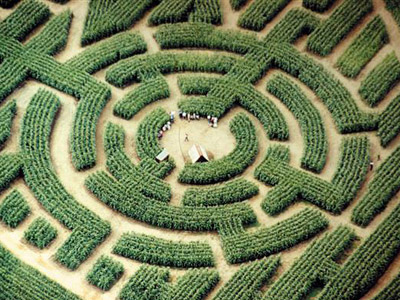
\includegraphics[width=4cm]{labyrinthe.jpg}
        \end{center}
	
\end{figure}


\section*{Introduction}

Le but de ce projet est d'étudier les \emph{labyrinthes} en tant qu'objets mathématiques et de chercher leurs différentes propriétés.

\textbf{Mots clés : combinatoire, énumération, algortihmes.}

Le principe du projet est d'étudier une question mathématique complexe de façon autonome et originale en utilisant l'outil informatique. \textbf{L'ensemble du projet est à faire par groupe de 3 étudiants.} Le projet est divisé en 2 sections : théorique et pratique. La première partie est \textbf{obligatoire}, la seconde partie correspond à des \textbf{pistes de travail}.

\subsection*{Rendu du projet}\strut

Vous devrez rendre:

\begin{itemize}

\item un \textbf{rapport de mi-projet} répondant aux questions de la section 1;

\item un \textbf{exposé} en fin de projet présentant votre travail et vos résultats sur la section 2.
\end{itemize}

\subsection*{Le rapport}\strut

\smallskip
\textbf{Date de rendu} : cf site du cours \url{https://www.lri.fr/~pons/teaching-mathinfo-l1.html}

\smallskip
\textbf{Que faut-il faire ?} Répondre aux questions de la section 1.

\smallskip
\textbf{Quel format ?} Format PDF obligatoire. Si vous souhaitez ajouter des dessins, vous pouvez les scanner et les ajouter à votre document.

\smallskip
\textbf{Qui réalise le rapport ?} Les membres du groupe réfléchissent ensemble au rapport mais rédigent chacun leur propre rapport. N'oubliez pas de préciser sur votre document qui sont les autres membres du groupe !

\smallskip
\textbf{Comment le rendre ?} Dans votre projet CoCalc, vous trouverez un dossier \og Rapport\fg, c'est là qu'il faut uploader votre rapport PDF.

\subsection*{L'exposé}\strut

\smallskip
\textbf{Quand ?} Les exposés auront lieu courant mai, la date sera précisée ultérieurement.

\smallskip
\textbf{Que doit-on présenter ?} Vous devez présenter le travail effecuté sur la section 2 du projet, en particulier les résultats que vous avez obtenus, les algorithmes que vous avez utilisés, les images ou vidéos produites, etc.

\smallskip
\textbf{En combien de temps ?} Vous aurez 10 minutes de présentation, puis 5 minutes de questions.

\smallskip
\textbf{Sur quel support ?} Vous aurez un vidéo projecteur et un ordinateur à disposition (ou le votre si vous le souhaitez). Vous pourrez donc présenter votre exposé sous forme d'un powerpoint ou pdf. Vous pouvez aussi montrer des images, vidéos, démos de code.

\smallskip
\textbf{Qui parle ?} Tout le monde ! Les 3 étudiants doivent participer.

\smallskip
\textbf{Doit-on présenter notre code ?} Vous pouvez utiliser un notebook CoCalc pour présenter des démos de code, cependant nous ne notons pas la programmation mais bien les résultats obtenus !

\smallskip
\textbf{Doit-on répondre aux questions ?} Les question de la section 2 ne sont pas obligatoires, ce sont des pistes de travail, vous pouvez les suivre, ou pas...


\section{\'Etude théorique du problème}

\subsection{Définitions}

On considère une grille rectangulaire de taille $n \times m$. Le bord du rectangle est appelé \emph{enceinte}, chaque case est appelée une \emph{cellule}. Des \emph{murs} peuvent être placés sur le côté des cellules. On appelle un ensemble \emph{enceinte}+\emph{murs} un \emph{pseudo-labyrinthe}, voir les exemples Figure \ref{ex:pseudo-labs}.

\begin{figure}[ht]
\begin{tabular}{cc}
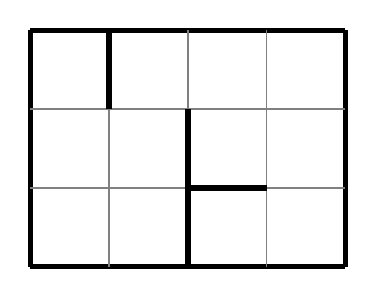
\begin{tikzpicture}
\draw[line width = 2](-0.5,0.5) -- (3.50000000000000,0.5);
\draw[line width = 2](-0.5,-2.50000000000000) -- (3.50000000000000,-2.50000000000000);
\draw[line width = 2](-0.5,0.5) -- (-0.5,-2.50000000000000);
\draw[line width = 2](3.50000000000000,0.5) -- (3.50000000000000,-2.50000000000000);
\draw[line width=0.5, color = gray](0.500000000000000, 0.5) -- (0.500000000000000,-2.50000000000000);
\draw[line width=0.5, color = gray](1.50000000000000, 0.5) -- (1.50000000000000,-2.50000000000000);
\draw[line width=0.5, color = gray](2.50000000000000, 0.5) -- (2.50000000000000,-2.50000000000000);
\draw[line width=0.5, color = gray](-0.5,-0.500000000000000) -- (3.50000000000000,-0.500000000000000);
\draw[line width=0.5, color = gray](-0.5,-1.50000000000000) -- (3.50000000000000,-1.50000000000000);
\draw[line width = 2](0.500000000000000,0.500000000000000) -- (0.500000000000000,-0.500000000000000);
\draw[line width = 2](1.50000000000000,-0.500000000000000) -- (1.50000000000000,-1.50000000000000);
\draw[line width = 2](1.50000000000000,-1.50000000000000) -- (1.50000000000000,-2.50000000000000);
\draw[line width = 2](1.50000000000000,-1.50000000000000) -- (2.50000000000000,-1.50000000000000);
\end{tikzpicture}
&
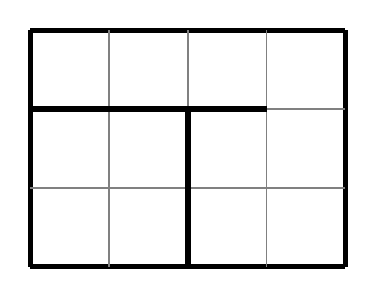
\begin{tikzpicture}
\draw[line width = 2](-0.5,0.5) -- (3.50000000000000,0.5);
\draw[line width = 2](-0.5,-2.50000000000000) -- (3.50000000000000,-2.50000000000000);
\draw[line width = 2](-0.5,0.5) -- (-0.5,-2.50000000000000);
\draw[line width = 2](3.50000000000000,0.5) -- (3.50000000000000,-2.50000000000000);
\draw[line width=0.5, color = gray](0.500000000000000, 0.5) -- (0.500000000000000,-2.50000000000000);
\draw[line width=0.5, color = gray](1.50000000000000, 0.5) -- (1.50000000000000,-2.50000000000000);
\draw[line width=0.5, color = gray](2.50000000000000, 0.5) -- (2.50000000000000,-2.50000000000000);
\draw[line width=0.5, color = gray](-0.5,-0.500000000000000) -- (3.50000000000000,-0.500000000000000);
\draw[line width=0.5, color = gray](-0.5,-1.50000000000000) -- (3.50000000000000,-1.50000000000000);
\draw[line width = 2](1.50000000000000,-0.500000000000000) -- (1.50000000000000,-1.50000000000000);
\draw[line width = 2](1.50000000000000,-1.50000000000000) -- (1.50000000000000,-2.50000000000000);
\draw[line width = 2](-0.500000000000000,-0.500000000000000) -- (0.500000000000000,-0.500000000000000);
\draw[line width = 2](0.500000000000000,-0.500000000000000) -- (1.50000000000000,-0.500000000000000);
\draw[line width = 2](1.50000000000000,-0.500000000000000) -- (2.50000000000000,-0.500000000000000);
\end{tikzpicture}

\end{tabular}
\caption{Deux exemples de pseudos-labyrinthes de taille $4 \times 3$}
\label{ex:pseudo-labs}
\end{figure}


Pour être un \emph{labyrinthe}, un pseudo-labyrinthe doit vérifier deux conditions:
\begin{enumerate}
\item l'espace à l'intérieur de l'enceinte est connexe: il existe toujours un chemin entre deux cellules données,
\label{cond:lab-connexe}
\item si l'on rajoute un mur où que ce soit, alors il perd sa connexité.
\label{cond:lab-max}
\end{enumerate}

\begin{figure}[ht]
\begin{tabular}{ccc}
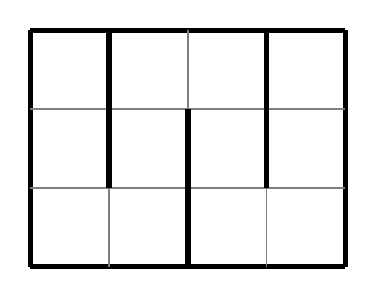
\begin{tikzpicture}
\draw[line width = 2](-0.5,0.5) -- (3.50000000000000,0.5);
\draw[line width = 2](-0.5,-2.50000000000000) -- (3.50000000000000,-2.50000000000000);
\draw[line width = 2](-0.5,0.5) -- (-0.5,-2.50000000000000);
\draw[line width = 2](3.50000000000000,0.5) -- (3.50000000000000,-2.50000000000000);
\draw[line width=0.5, color = gray](0.500000000000000, 0.5) -- (0.500000000000000,-2.50000000000000);
\draw[line width=0.5, color = gray](1.50000000000000, 0.5) -- (1.50000000000000,-2.50000000000000);
\draw[line width=0.5, color = gray](2.50000000000000, 0.5) -- (2.50000000000000,-2.50000000000000);
\draw[line width=0.5, color = gray](-0.5,-0.500000000000000) -- (3.50000000000000,-0.500000000000000);
\draw[line width=0.5, color = gray](-0.5,-1.50000000000000) -- (3.50000000000000,-1.50000000000000);
\draw[line width = 2](0.500000000000000,0.500000000000000) -- (0.500000000000000,-0.500000000000000);
\draw[line width = 2](0.500000000000000,-0.500000000000000) -- (0.500000000000000,-1.50000000000000);
\draw[line width = 2](1.50000000000000,-0.500000000000000) -- (1.50000000000000,-1.50000000000000);
\draw[line width = 2](1.50000000000000,-1.50000000000000) -- (1.50000000000000,-2.50000000000000);
\draw[line width = 2](2.50000000000000,0.500000000000000) -- (2.50000000000000,-0.500000000000000);
\draw[line width = 2](2.50000000000000,-0.500000000000000) -- (2.50000000000000,-1.50000000000000);
\end{tikzpicture}
&
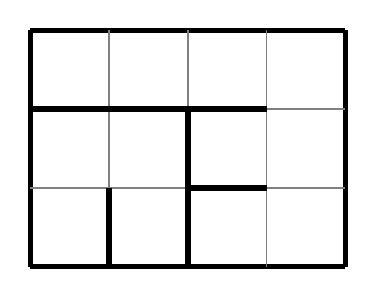
\begin{tikzpicture}
\draw[line width = 2](-0.5,0.5) -- (3.50000000000000,0.5);
\draw[line width = 2](-0.5,-2.50000000000000) -- (3.50000000000000,-2.50000000000000);
\draw[line width = 2](-0.5,0.5) -- (-0.5,-2.50000000000000);
\draw[line width = 2](3.50000000000000,0.5) -- (3.50000000000000,-2.50000000000000);
\draw[line width=0.5, color = gray](0.500000000000000, 0.5) -- (0.500000000000000,-2.50000000000000);
\draw[line width=0.5, color = gray](1.50000000000000, 0.5) -- (1.50000000000000,-2.50000000000000);
\draw[line width=0.5, color = gray](2.50000000000000, 0.5) -- (2.50000000000000,-2.50000000000000);
\draw[line width=0.5, color = gray](-0.5,-0.500000000000000) -- (3.50000000000000,-0.500000000000000);
\draw[line width=0.5, color = gray](-0.5,-1.50000000000000) -- (3.50000000000000,-1.50000000000000);
\draw[line width = 2](0.500000000000000,-1.50000000000000) -- (0.500000000000000,-2.50000000000000);
\draw[line width = 2](1.50000000000000,-0.500000000000000) -- (1.50000000000000,-1.50000000000000);
\draw[line width = 2](1.50000000000000,-1.50000000000000) -- (1.50000000000000,-2.50000000000000);
\draw[line width = 2](-0.500000000000000,-0.500000000000000) -- (0.500000000000000,-0.500000000000000);
\draw[line width = 2](0.500000000000000,-0.500000000000000) -- (1.50000000000000,-0.500000000000000);
\draw[line width = 2](1.50000000000000,-0.500000000000000) -- (2.50000000000000,-0.500000000000000);
\draw[line width = 2](1.50000000000000,-1.50000000000000) -- (2.50000000000000,-1.50000000000000);
\end{tikzpicture}
&
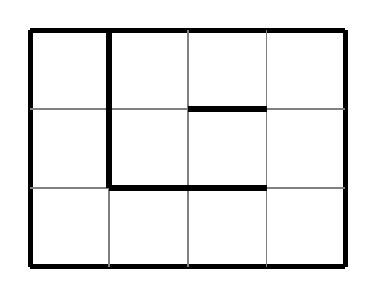
\begin{tikzpicture}
\draw[line width = 2](-0.5,0.5) -- (3.50000000000000,0.5);
\draw[line width = 2](-0.5,-2.50000000000000) -- (3.50000000000000,-2.50000000000000);
\draw[line width = 2](-0.5,0.5) -- (-0.5,-2.50000000000000);
\draw[line width = 2](3.50000000000000,0.5) -- (3.50000000000000,-2.50000000000000);
\draw[line width=0.5, color = gray](0.500000000000000, 0.5) -- (0.500000000000000,-2.50000000000000);
\draw[line width=0.5, color = gray](1.50000000000000, 0.5) -- (1.50000000000000,-2.50000000000000);
\draw[line width=0.5, color = gray](2.50000000000000, 0.5) -- (2.50000000000000,-2.50000000000000);
\draw[line width=0.5, color = gray](-0.5,-0.500000000000000) -- (3.50000000000000,-0.500000000000000);
\draw[line width=0.5, color = gray](-0.5,-1.50000000000000) -- (3.50000000000000,-1.50000000000000);
\draw[line width = 2](0.500000000000000,0.500000000000000) -- (0.500000000000000,-0.500000000000000);
\draw[line width = 2](0.500000000000000,-0.500000000000000) -- (0.500000000000000,-1.50000000000000);
\draw[line width = 2](0.500000000000000,-1.50000000000000) -- (1.50000000000000,-1.50000000000000);
\draw[line width = 2](1.50000000000000,-0.500000000000000) -- (2.50000000000000,-0.500000000000000);
\draw[line width = 2](1.50000000000000,-1.50000000000000) -- (2.50000000000000,-1.50000000000000);
\end{tikzpicture}\\
(a)
&
(b)
&
(c)
\end{tabular}
\caption{Exemple et contre-exemples de labyrinthes}
\label{fig:laby}
\end{figure}

Dans la figure \ref{fig:laby}, seul (a) est un labyrinthe. En effet, (b) ne satisfait pas la condition \eqref{cond:lab-connexe} et (c) ne vérifie pas la condition \eqref{cond:lab-max}.


\subsection{Questions}

\begin{enumerate}

\item Dessinez tous les pseudo-labyrinthes de taille $2 \times 2$ (vous devez en trouver 16). Combien sont des labyrinthes ? 

\item Quel est le nombre maximal de murs dans un pseudo-labyrinthe de taille $n \times m$ ?

\item Si $m=1$, combien existe-t-il de pseudo labyrinthme de taille $n \times 1$ ?

\item Observez les cas $m=2$ et $m=3$ et donnez la formule générale pour le nombre de pseudo labyrinthe de taille $n \times m$ en justifiant votre réponse.

\item Dessinez tous les labyrinthes de taille $3 \times 2$. Vous devez en trouver 15. 

\item En comptant les murs de chacun de ces labyrinthes, que remarquez-vous ? 

\item Soit $L$ un labyrinthe, on suppose que la sortie se trouve dans la cellule en haut à gauche. Prouvez que si je choisis une cellule $c$ quelconque de $L$, alors il existe un unique chemin qui va de $c$ à la sortie sans passer plus d'une fois sur chacune des cases (il faut prouver que ce chemin existe et qu'il est unique). 


\item En utilisant le résultat précédent, il est possible de prouver que pour un labyrinthe de taille $n \times m$, il existe exactement $n \times m - 1$ bordures entre cellules qui ne sont pas des murs (on ne vous demande pas la preuve). Un pseudo-labyrinthe possédant le "bon" nombre de murs est-il toujours un labyrinthe ? Conjecturez une condition nécessaire et suffisante pour qu'un pseudo-labyrinthe soit un labyrinthe. 

\end{enumerate}

\section{Modélisation et exploration}

Le problème mathématique que nous avons présenté ici sous forme de labyrinthes est un véritable problème de recherche qui pose de nombreuses questions. Certaines de ces questions n'ont pas de réponses à ce jour ! Le but de ce projet est maintenant d'explorer ces questions par vous même en utilisant l'outil informatique. Il n'y a pas de solution unique, ni même de direction imposée, nous vous proposons simplement des pistes...

\subsection{Modélisation et visualisation}

La première étape consiste à représenter les objets "pseudo-labyrinthe" et "labyrinthes" par des objets informatiques.

\begin{enumerate}
\item Quelle structure de donnée pouvez-vous utiliser pour représenter un pseudo-labyrinthe~?

\item Comment pouvez-vous tester si un pseudo-labyrinthe est un labyrinthe ? (Et quelle est la complexité de l'algorithme)

\item Implantez une méthode pour "dessiner" un pseudo-labyrinthe représenté par votre structure de donnée (utilisez la méthode \emph{plot}).
\end{enumerate}

Quelques pistes : les tableaux et matrices vous sembleront peut-être les objets les plus évidents, vous pouvez aussi regarder du coté des \emph{graphes}.

\subsection{Génération aléatoire}

Réfléchissez à des algorithmes pour générer des pseudo-labyrinthes et labyrinthes de façon aléatoire. Implantez et testez vos algorithmes et répondez à certaines questions du type :

\begin{enumerate}
\item La génération est-elle uniforme (chaque labyrinthe apparaît avec la même probabilité) ?

\item Quelle est la complexité de votre algorithme ?

\item \'A quoi "ressemblent" de très gros pseudo-labyrithes ou labyrinthes tirés aléatoirement ?
\end{enumerate}

\subsection{\'Enumération}

Le but de cette section est d'étudier la question du nombre de labyrinthes pour des valeurs de $n$ et $m$ données.

\begin{enumerate}
\item (difficile) Proposez et implantez un algorithme pour générer l'ensemble des labyrinthes d'une taille $n\times m$ donnée. \textbf{Donc votre algorithme doit retourner la liste des labyrinthes possible.}

\item Vérifiez par des tests sur différentes valeurs les résultats prouvés et conjecturés dans la partie théorique.

\item Affichez dans un tableau à double entrée le nombre de labyrinthes de taille $n \times m$ en faisant varier $n$ et $m$ (voyez comment évoluent les nombres et jusqu'où vous pouvez aller). Chaque ligne (ou chaque colonne) du tableau vous donne une liste de nombre que vous pouvez étudier. 

\item Existe-t-il d'autres moyens de calculer ces nombres que par la génération de tous les labyrinthes~? Intéressez vous aux notions d'arbres couvrants (ou \emph{spanning trees}) et aux algorithmes existants et implantés dans Sage. 

\item On joue à "quel est le prochain nombre" : comprendre la logique d'une suite de nombres et "deviner" la suite. Pour cela, on peut utiliser le site \url{http://www.oeis.org} qui référence les suites de nombres connues. Cherchez sur ce site les différentes formules existantes pour calculer les nombre du tableau. 

\item La première ligne intéressante du tableau est celle pour $n=2$. Dans ce cas la formule récursive est relativement simple (cherchez la sur \url{http://www.oeis.org}). Vous pouvez essayer de la "comprendre" : prenez un labyrinthe de taille $2 \times 3$ de votre choix et rajouter 2 cellules pour obtenir un pseudo-labyrinthe de taille $2 \times 4$, comment en faire un labyrinthe ? Comment obtenir tous les labyrinthes de taille $2 \times 4$ à partir des labyrinthes de taille $2 \times 3$ ?
\end{enumerate}


\subsection{D'autres directions...}

Ce problème a été posé lors du tournoi des jeunes mathématiciennes et mathématiciens 2014. Vous trouverez sur le site du tournoi, \url{http://www.tfjm.org} d'autres pistes de recherche sur les labyrinthes.

\vspace{2cm}
\footnotesize{Image : Labyrinthe de Barvaux, \url{https://commons.wikimedia.org/wiki/File:Labyrint_barvaux.jpg}}

\end{document}

